
\section{Case study: Erythropoietin signal transduction}

We tested our approach to optimal experiment design using the model of the
Erythropoietin signal transduction in the cell line \texttt{HEK293} derived from
human embryonic kidney cells.
Erythropoietin (Epo) is a cytokine which initiates red blood cell generation and
thus adjusts the capacity of the blood to transport oxygen.
The Epo-encoding gene is activated in case of hypoxia in the kidney and liver by
the transcription factor HIF (hypoxia induced factor).
Epo acts on erythroid progenitor cells which finally develop to reticulocytes\cite{wib1}.
This differentiation depends on binding of Epo to the transmembrane Epo receptor.
The receptor does not harbour intrinsic kinase activity but is constitutively
associated with the tyrosine kinase JAK2 (Janus kinase 2).
After binding of Epo to the receptor, JAK2 is tyrosine phosphorylated and thus activated.
JAK2 subsequently phosphorylates and activates the transcription factors signal
transducer and activator of transcription (STAT)3 and 5.
A negative feedback is implemented by the induction of the STAT-dependent feedback
inhibitors SOCS3 and CIS\cite{wib2}.
The regulation of the STAT-independent signalling modules involves the multi-site
docking proteins of the Gab (Grb2 associated binder) family\cite{wib3}.
Gab-proteins contribute to the coordination and activation of the PI3K/AKT pathway,
the MAPK-cascade, and the PLC-cascade.
The detailed interconnection of these signalling modules is not fully understood, yet.
In brief, Gab proteins are recruited to the plasma membrane and there act as a
signalling platform by binding Grb2/SOS, SHP2, PI3K, PLC and other signalling
components.
Several regulatory loops are predicted as e.g. Gab binding to PIP3 in the plasma
membrane depends on PI3K- and MAPK-activity\cite{wib4}.
The original model that served as our gold standard was given in form of a
Boolean network (BN).
The hypergraph representation of the Boolean network contains $23$ species and
$28$ hyperarcs.
In Boolean networks the underlying interaction graphs can easily be obtained\cite{sk06}.

A realistic experimental setup involves the following list of possible
perturbations and readouts.
\begin{itemize}
  \item
  nine possible down-regulations (e.g.\ by use of suitable inhibitors):
  {\sffamily akt},
  {\sffamily mek1},
  {\sffamily mtorc1},
  {\sffamily pi3k},
  {\sffamily gab1\_ps},
  {\sffamily gab1\_bras\_py},
  {\sffamily gab1\_bpi3k\_py},
  {\sffamily shp2, shp2\_ph},
  \item
  three possible up-regulations:
  {\sffamily gab1\_ps},
  {\sffamily shp2},
  {\sffamily shp2\_ph}, and
  \item eight possible readouts:
  {\sffamily akt},
  {\sffamily erk},
  {\sffamily gab1\_bshp2\_ph\_py},
  {\sffamily gab1\_ps},
  {\sffamily jak2\_p},
  {\sffamily plcg},
  {\sffamily shp2},
  {\sffamily stat5ab\_py}.\end{itemize}

In the first part of this case study,
we used \emph{in silico} experiments to validate our approach by creating a
distorted version of the gold standard and then planning experiments that
restored the gold standard.
In the second part, we planned \emph{in vivo} experiments to refine our
knowledge of the Erythropoietin signaling pathway in \texttt{HEK293} cells.


\subsection{\emph{In silico} experiments}

We tested our approach \emph{in silico} by restoring the gold standard model
of the Erythropoietin signal transduction from a distorted version of the model.
We performed quantitative simulations of the proposed experiments using an
ODE system which was created from the gold standard.
A detailed description of the \emph{in silico} study is given in the following:

\begin{itemize}
  \item First, we created an ODE system from the gold standard BN using the software ODEfy\cite{odefy}.
  \item This ODE model of the gold standard was used to simulate three initial experiments and subsequently
the experiments that were proposed by our experiment design procedure.

We identified a steady state in the ODE system,
which we used as initial state of the system in our simulated experiments.
In order to simulate the perturbation at time point 0,
we fixed the variables for the perturbed species to constants such that
increased species had a value significantly higher than in the initial state,
decreased species a value %$0.1$ times the value
significantly lower than in initial state, and
0-perturbed species were kept constant as in the initial state.
We restarted the simulation using these perturbed values and tracked the sign
of the first change of the dependent system variables as initial response.
%\comment{Sven: Add after how much time, how many timesteps? parameters of steady-state!}

The three initial experiments were
1) an increase of {\sffamily mek1},
2) a decrease of {\sffamily pi3k}, and
3) the simultaneous decrease of {\sffamily mek1} and {\sffamily pi3k}.

  \item As starting point for experiment planning and model reconstruction,
we transformed the gold standard BN into an influence graph which consists of
 $23$ nodes and $51$ edges (Figure~\ref{fig:goldVSdistorted}a).
%The compressed IG model consisted of
% $23$ nodes and $51$ edges.
We then created a distorted version (Figure~\ref{fig:goldVSdistorted}b) where
we removed the edge ({\sffamily erk} $\rightarrow$ {\sffamily gab1\_ps}) and added two new edges
 ({\sffamily mek1} $\dashv$ {\sffamily shp2}) and
 ({\sffamily mek1} $\rightarrow$ {\sffamily stat5ab\_py}).
%\comment{Wiebke:Ist es notwendig zu erläutern was gab1\_ps oder stat5ab-py und später folgende bedeuten?}
%\comment[Sven: nur auf nachfrage!}
These wrong/missing edges needed to be identified by the inference method.
%The influence graph of the gold standard model and the distorted version are
%shown side by side in Figure~\ref{fig:goldVSdistorted}.



%  \item We used the ODE model of the gold standard to simulate three
%realistic experiments.
%As expected the results of the simulated experiment were consistent with our
%IG model of the gold standard but inconsistent with the distorted IG model.

  \item We used the OPT\_GRAPH method for network inference on the distorted model
together with the data of the initial experiments.
As expected the data of the simulated experiment were consistent with our
gold standard but inconsistent with the distorted IG model.
OPT\_GRAPH proposed six candidate models that were consistent with the initial experiment data.
Note, that in our case the gold standard IG was among those candidate models,
which is not guaranteed by the OPT\_GRAPH method.

  \item We started the first round of experiment planning,
with these six candidate models including the constraints on possible perturbations and
readouts.
In the first round an experimental setup with one perturbation (decrease of {\sffamily akt} via {\sffamily akt\_inhibitor}) was proposed.
Figure~\ref{tab:predictions_allexp} shows the predicted behaviors
for the six network candidates in the proposed experiment.
The simulation results of the proposed experiment were consistent with three
models (4, 5, 6) and could exclude three candidates (1, 2, 3).

  \item In the second round of experiment planning two experiments with two perturbations
distinguishing two classes of models were proposed.
Figure~\ref{tab:predictions_allexp} shows the predicted behaviors for one of
the proposed experiments (simultaneous decrease of {\sffamily gab1\_bras\_py} and {\sffamily shp2}).
The simulation results of the proposed experiment were consistent with two
models (4, 5) and could exclude one candidate (6).

This point marks the limit of what is currently technically possible.
We have had exhausted all the perturbation and measuring methods available to
the wet lab.
It would not be possible to distinguish the remaining models.
However our ODE model does not succumb to these restrictions as we can observe
and perturb all components.

  \item We continued the third round of experiment planning dropping all restrictions
on possible perturbations.
Two experiment setups distinguishing the maximal number of two classes of models
with the minimum of two perturbations were proposed.
The Figure~\ref{tab:predictions_allexp} shows the predicted behaviors for one of
the proposed experiments (simultaneous increase of {\sffamily erk} and decrease of {\sffamily mek}).
Finally, the predictions of only one model is consistent with the results of
the simulated experiment,
model $5$ which is identical to our gold standard.

\end{itemize}

\begin{figure}[h]
\begin{center}
 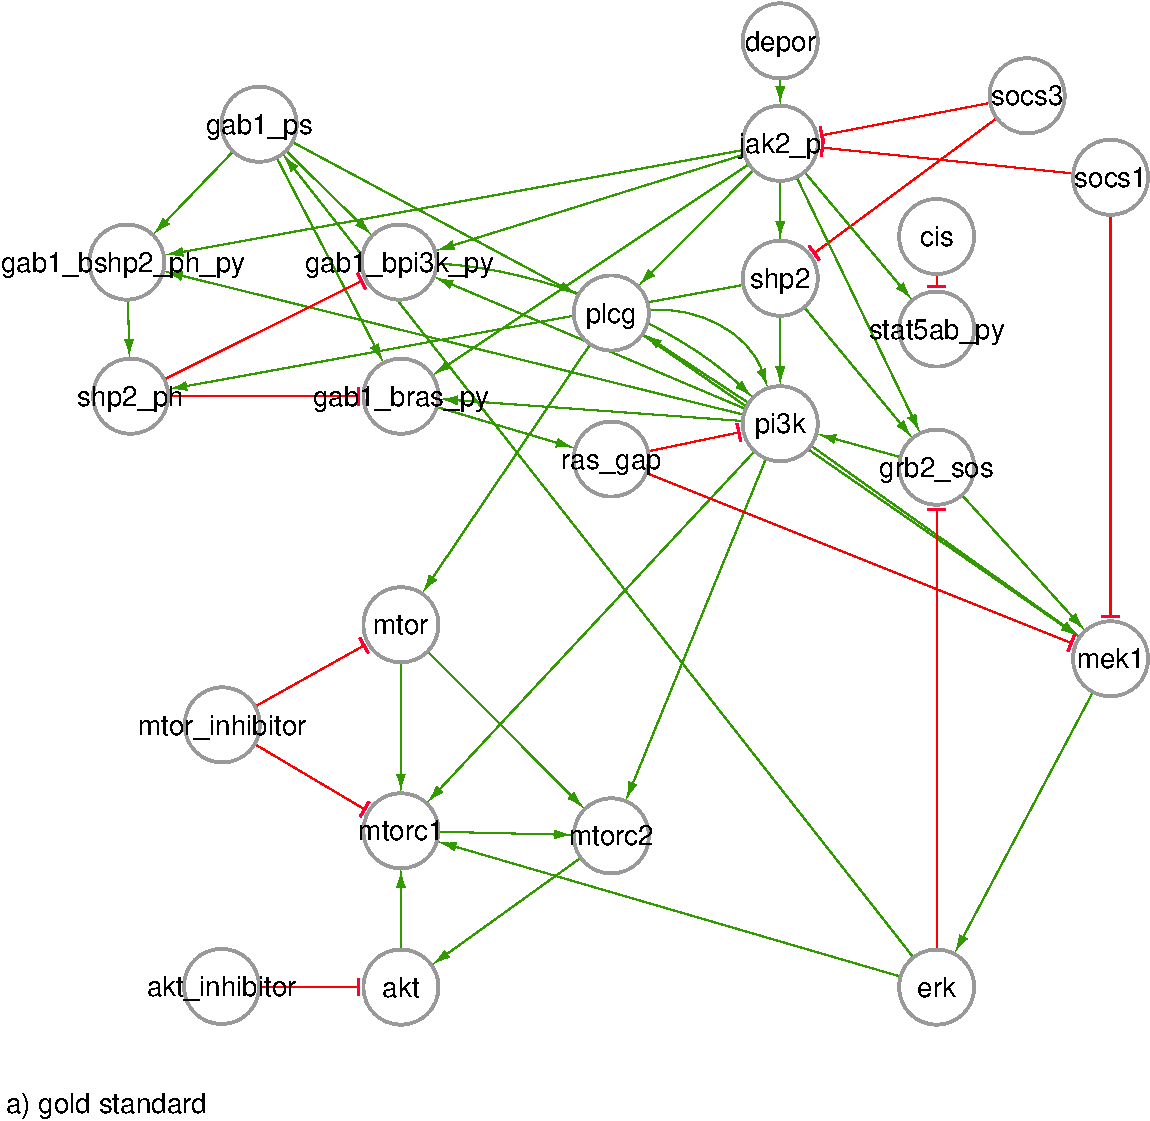
\includegraphics[scale=.45,keepaspectratio=true]{./figures/gold_standard_IG.pdf}
 ~~~
 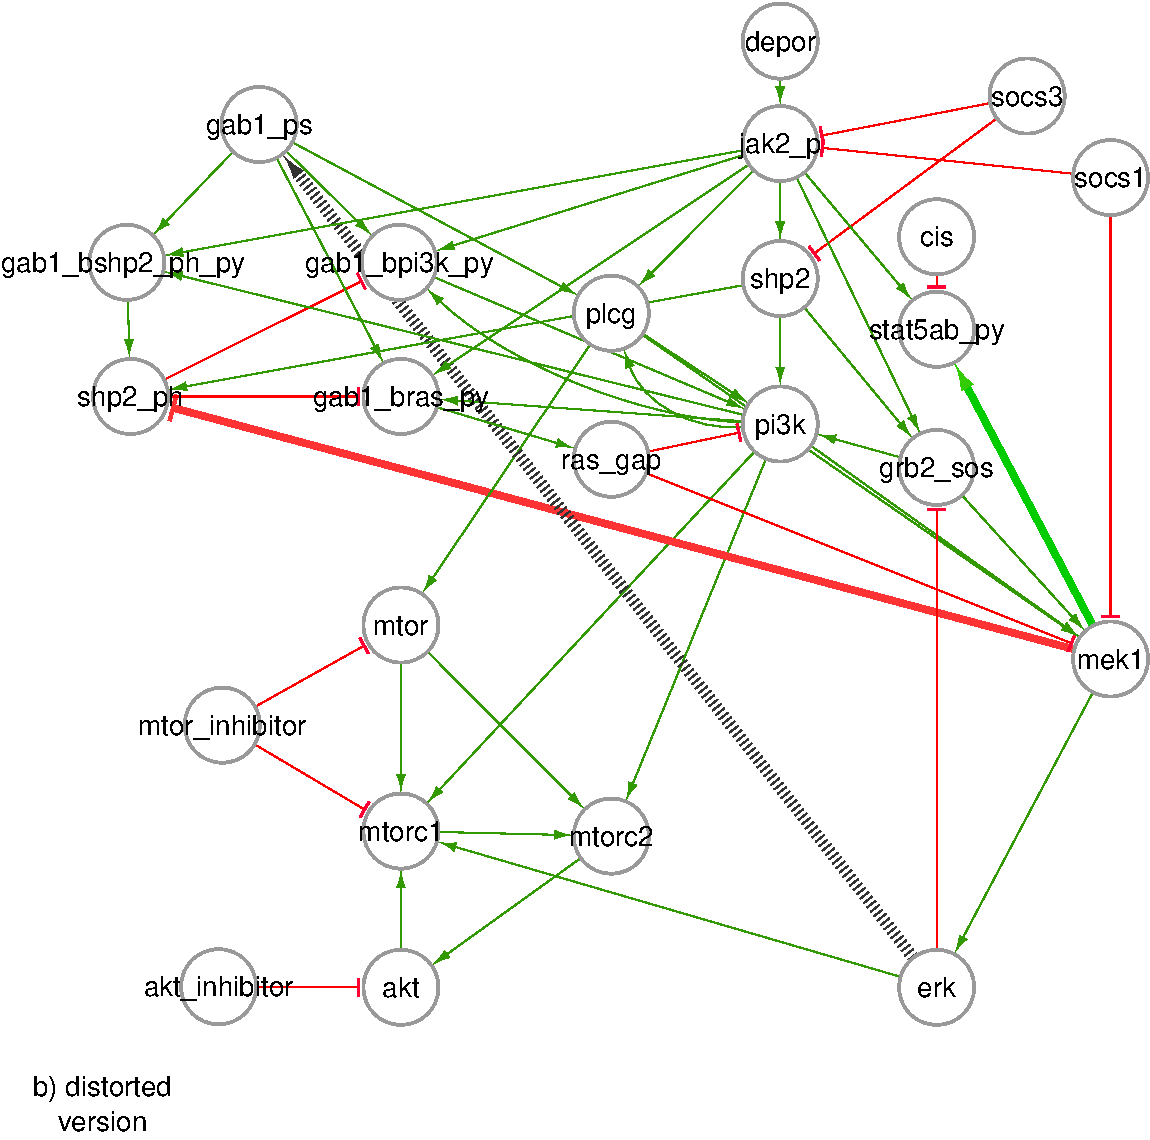
\includegraphics[scale=.45,keepaspectratio=true]{./figures/distorted_IG.pdf}

 \caption{
   The influence graph model of the gold standard (a) and the distorted version (b).
   Added edges are drawn thicker and removed edges are striked out.
 }
 \label{fig:goldVSdistorted}
\end{center}
\end{figure}

\begin{figure}[h]
\begin{center}
\sffamily
\small
\begin{tabular}{c|c|c| c|c|c| c|c|c|}
~ & \multicolumn{2}{c|}{Experiment 1} & \multicolumn{3}{c|}{Experiment 2} & \multicolumn{3}{c|}{Experiment 3} \\
~ & pert. & read & \multicolumn{2}{c|}{pert.} & read & \multicolumn{2}{c|}{pert.} & read \\
  model id & \rot{akt\_inhibitor} &  \rot{gab1\_ps}
           & \rot{gab1\_bras\_py} & \rot{shp2} &\rot{gab1\_ps}
           & \rot{erk} & \rot{mek1} & \rot{gab1\_ps} \\
  \hline
5 & $\plus$ & \gc  0       & $\minus$ & $\minus$ & \gc \am & $\plus$ & $\minus$ & \gc $\plus$  \\
4 & $\plus$ & \gc  0       & $\minus$ & $\minus$ & \gc \am & $\plus$ & $\minus$ & \rc $\minus$ \\
% \cline{11-13}
6 & $\plus$ & \gc  0       & $\minus$ & $\minus$ & \rc $\plus$ & \multicolumn{3}{c|}{~} \\
% \cline{8-10}
1 & $\plus$ & \rc $\minus$ & \multicolumn{3}{c|}{~} & \multicolumn{3}{c|}{~} \\
2 & $\plus$ & \rc $\minus$ & \multicolumn{3}{c|}{~} & \multicolumn{3}{c|}{~} \\
3 & $\plus$ & \rc $\minus$ & \multicolumn{3}{c|}{~} & \multicolumn{3}{c|}{~} \\
\hline
  \multicolumn{1}{c}{~} \\
  \multicolumn{2}{c}{~} & \multicolumn{7}{c}{simulation results} \\
  \cline{3-3}\cline{6-6}\cline{9-9}
  \multicolumn{2}{l|}{gold standard} & 0 & \multicolumn{2}{c|}{~} & $\minus$ & \multicolumn{2}{c|}{~} & $\plus$\\
  \cline{3-3}\cline{6-6}\cline{9-9}
\end{tabular}
\end{center}
\caption{
  Results of the \emph{in silico} study. Predicted behavior for the candidate models and behavior of the
  gold standard simulation under the proposed experiment.
  Predictions that are consistent with the simulation results are in green,
  inconsistent predictions are shown red.
}
\label{tab:predictions_allexp}
\end{figure}


\subsection{\emph{In vivo} experiments}

For \emph{in vivo} experimentation,
we started with $26$ model candidates based on the gold standard and existing
experimental data\footnote{online available at:\\ https://github.com/bioasp/iggy/tree/master/data/in\_vivo\_HEK293}.
%\comment{Wiebke: Welche Daten sind das? Ist dafür auch eine genauere Beschreibung notwendig?}
%\comment{Sven: create supplements! Beschreibung nur auf Nachfrage!}
Our experiment planning proposed the experiment shown in Figure~\ref{tab:predictionsWt}
in which the inhibition of {\sffamily akt} would allow us to distinguish two classes
of models and thus to invalidate at least six model candidates.
%
These model classes are illustrated in Figure~\ref{fig:modeltypeAB1}.
All model candidates suggest to introduce a regulation of {\sffamily erk} that was not
present in the gold standard.
The models of class $A$ contain regulations upstream of {\sffamily akt} via
 {\sffamily gab1\_bshp2\_ph\_py},
 {\sffamily gab1\_bpi3k\_py},
 {\sffamily plcg},
 {\sffamily gab1\_bras\_py},
 {\sffamily ras\_gap},
 {\sffamily pi3k} or
 {\sffamily mtor}.
If a model from class $A$ reflects the biological reality,
then an inhibition of {\sffamily akt} should have no effect on {\sffamily erk}.
The models of class $B$ contain a regulation of {\sffamily erk} downstream of
{\sffamily akt}, via
 {\sffamily mtorc1},
 {\sffamily mtorc2} or
 {\sffamily akt} directly.
If a model of class $B$ reflects reality we should see an increase in
{\sffamily erk} and {\sffamily gab1\_ps}.

\begin{figure}[h]
\begin{center}
\sffamily
\small
\begin{tabular}{c|c| c|c|c|c|c|c|}
~ & \multicolumn{1}{c|}{pert.} & \multicolumn{6}{c|}{readout} \\
model id & akt\_inhibitor & \rot{erk} & \rot{jak2\_p} & \rot{plcg} & \rot{gab1\_ps} & \rot{stat5ab\_py} & \rot{shp2} \\
\hline
Class A   &          &         &     &     &         &     &     \\
20 models & $\plus$ &       0 &  0  &  0  & 0       &  0  &  0  \\
          &          &         &     &     &         &     &     \\
Class B   &          &         &     &     &         &     &     \\
6 models  & $\plus$ & $\plus$ & \am & \am & $\plus$ & \am & \am \\

\end{tabular}
\end{center}
\caption{
  Predicted behavior for the candidate models of the Erythropoietin signal
  transduction in \texttt{HEK293} cells in Experiment~1 of the \emph{in vivo} study.
}
\label{tab:predictionsWt}
\end{figure}

\begin{figure}[h]
\begin{center}
 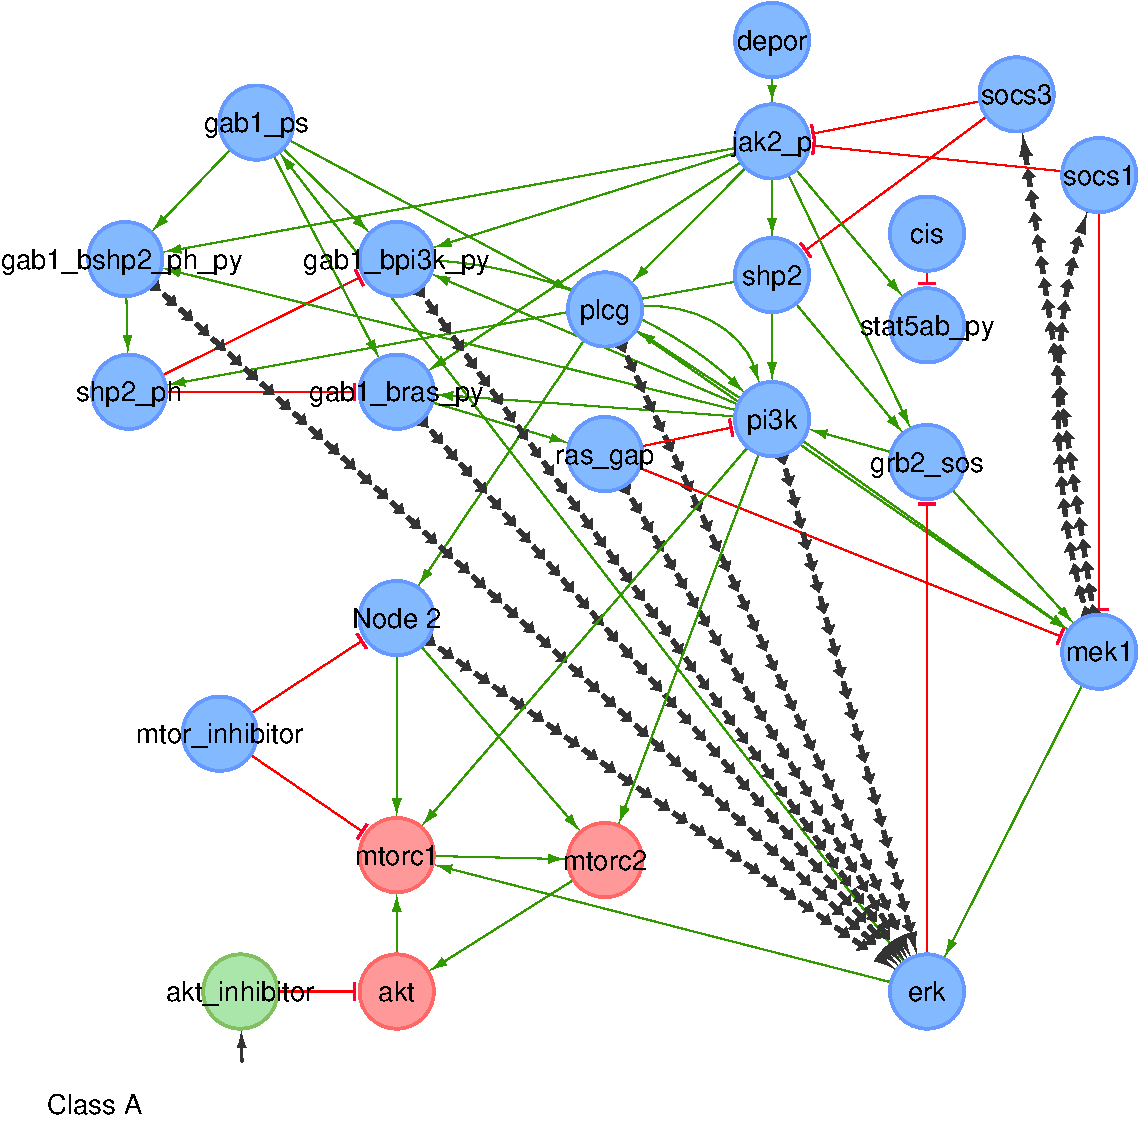
\includegraphics[scale=.45,keepaspectratio=true]{./figures/wt_model_class_A.pdf}

 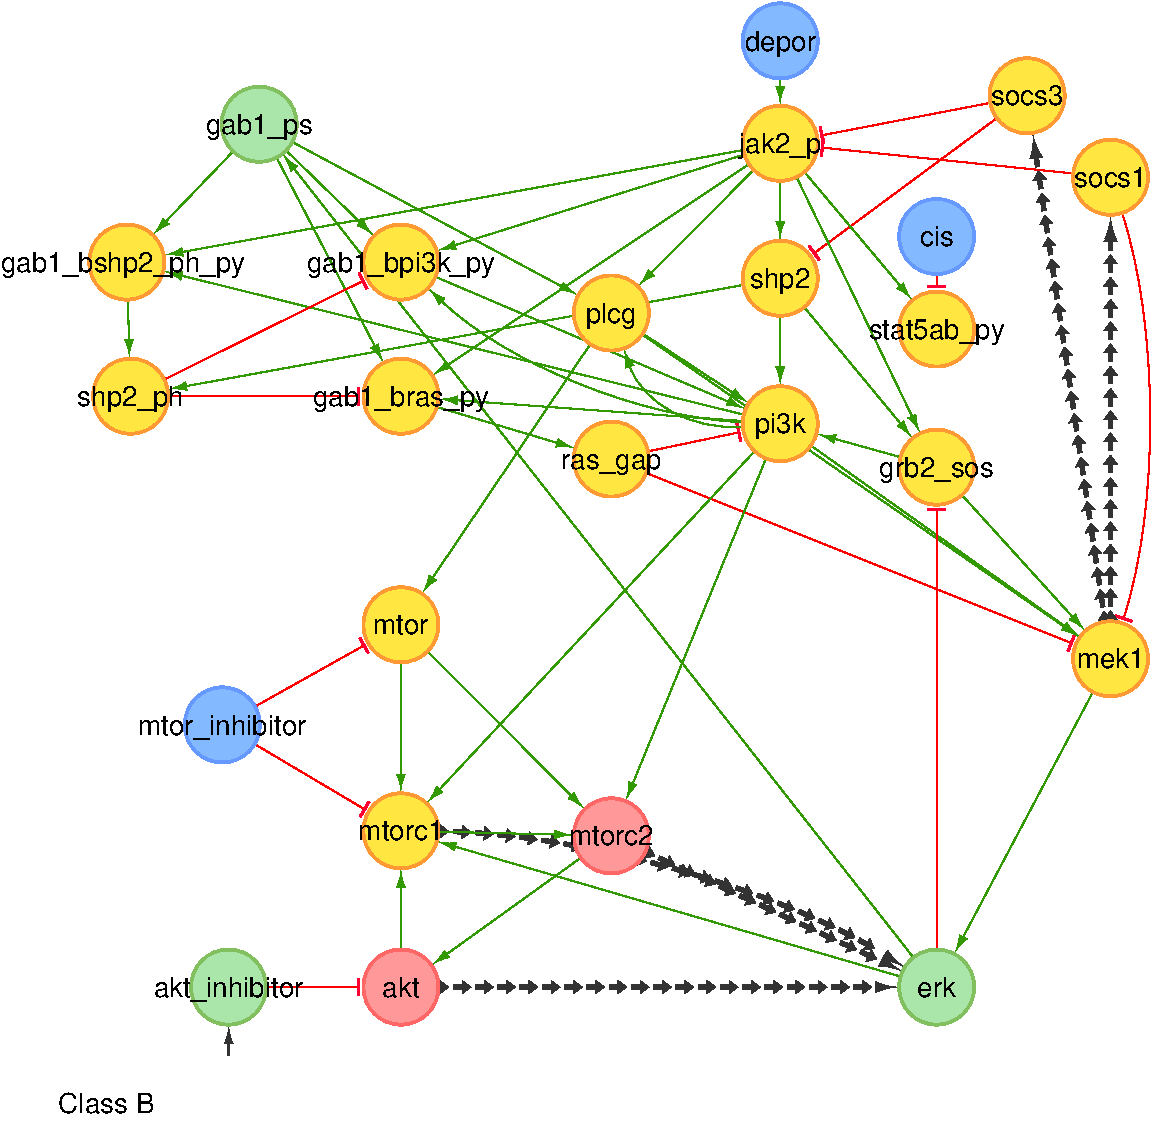
\includegraphics[scale=.45,keepaspectratio=true]{./figures/wt_model_class_B.pdf}
 \end{center}
 \caption{
   Two model classes for the Erythropoietin signal transduction network in \texttt{HEK293} cells.
   Alternative regulations in different models are shown with black arrows.
   Class $A$ contains regulations of {\sffamily erk} upstream of {\sffamily akt}.
   Class $B$ contains regulations of {\sffamily erk} downstream of {\sffamily akt}.
   Models of class $A$ predict no effect of an inhibition of {\sffamily akt},
   while models of class $B$ predict an increase of {\sffamily erk} and {\sffamily gab1\_ps}.
 }
 \label{fig:modeltypeAB1}
\end{figure}

The experiment was set up and performed according to the computed specification.
\texttt{HEK293} cells expressing JAK2 wild type and the Epo receptor were pre-treated
with the Akt inhibitor MK-2206 (2 $\upmu$M, 30 min) or solvent control before Epo
stimulation (3 U/ml, 15 min).
Cell lysates were prepared and proteins were separated by SDS–PAGE.
After Western blotting, the membranes were stained for phosphorylated forms of
Gab1, JAK2, STAT5, PLC$\upgamma$, SHP2, Erk1/2 and Akt.
Three independent experiments were performed.
The experimental results showed that the inhibition of {\sffamily akt} had no
effect on {\sffamily erk} and {\sffamily gab1\_ps}.
Therefore, we were able to exclude six of the model candidates and perform
a second round of experiment planning trying to discriminate among the remaing
$20$ model candidates.

In the second round our experiment planning proposed the experiment shown in
Figure~\ref{tab:predictionsWt2}.
The proposed inhibition of {\sffamily mtor} distinguished two classes of models.
Promising to invalidate at least two of the model candidates.
The models of class $C$ contain regulations upstream of {\sffamily mtor} via
 {\sffamily gab1\_bshp2\_ph\_py},
 {\sffamily gab1\_bpi3k\_py},
 {\sffamily plcg},
 {\sffamily gab1\_bras\_py},
 {\sffamily ras\_gap} or
 {\sffamily pi3k}.
If a model from class $C$ reflects the biological reality,
then an inhibition of {\sffamily mtor} should have no effect on {\sffamily erk}.
The models of class $D$ contain a regulation of {\sffamily erk} via
{\sffamily mtor}.
If a model of class $D$ reflects reality we should see an increase in
{\sffamily erk} and {\sffamily gab1\_ps}.

\begin{figure}[h]
\begin{center}
\sffamily
\small
\begin{tabular}{c|c| c|c|c|c|c|c|}
~ & \multicolumn{1}{c|}{pert.} & \multicolumn{6}{c|}{readout} \\
model id & {mtor\_inhibitor} & \rot{erk} & \rot{jak2\_p} & \rot{plcg} & \rot{gab1\_ps} & \rot{stat5ab\_py} & \rot{shp2} \\
\hline
Class C   &         &         &     &     &         &     &     \\
18 models & $\plus$ &       0 &  0  &  0  & 0       &  0  &  0  \\
          &         &         &     &     &         &     &     \\
Class D   &         &         &     &     &         &     &     \\
2 models  & $\plus$ & $\plus$ & \am & \am & $\plus$ & \am & \am \\
\end{tabular}
\end{center}
\caption{
  Predicted behavior for the candidate models of the Erythropoietin signal
  transduction in \texttt{HEK293} cells in Experiment~2 of the \emph{in vivo} study.
}
\label{tab:predictionsWt2}
\end{figure}

The experiment was set up and performed according to the computed specification.
\texttt{HEK293} cells expressing JAK2 wild type and the Epo receptor were pre-treated
with the mTOR inhibitor Rapamycin (10 nM, 30 min) or solvent control before Epo
stimulation (3 U/ml, 15 min).
Cell lysates were prepared and proteins were separated by SDS–PAGE.
After Western blotting, the membranes were stained for phosphorylated forms of
Gab1, JAK2, STAT5, PLC$\upgamma$, SHP2, Erk1/2 and Akt.
Three independent experiments were performed.
The experimental results showed that the inhibition of {\sffamily mtor} had
no effect on our readout species.
Therefore, we were able to exclude another two of the model candidates reducing
the candidate set to $18$.

Continued experiment planning proposed further experiments that contained
multiple perturbations which, however, were too complex to conduct with our
facilities.


\subsection{Testing scalability and sensitivity }

To assess the sensitivity and scalability of our approach with respect to different settings
we created 165 distorted models from the gold standard (Figure~\ref{fig:goldVSdistorted}a).
In each distorted model, 1 edge from the gold standard has been deleted and 2 edges not contained
in the gold standard have been added.
For each distorted model we used the OPT\_GRAPH method together with the existing real experimental data
and computed candidate models that correct the inconsistencies with the experimental data.
Figure~\ref{fig:candidates} shows a histogram for the number of candidate models that have been proposed
for the distorted models.

\begin{figure}[h]
\begin{center}
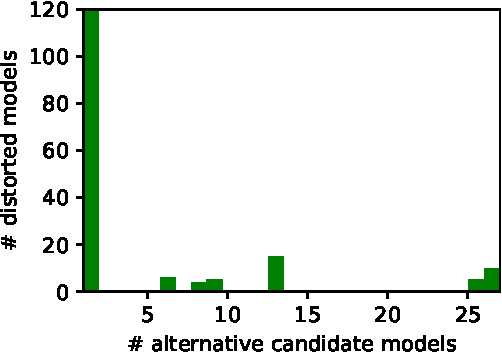
\includegraphics[scale=0.9,keepaspectratio=true]{./figures/histogram.pdf}
\end{center}
\caption{
 Number of candidate models proposed for each of the 165 distorted models.
 For 120 distorted models, OPT\_GRAPH proposed a single candidate model
 while for the remaining 45 distorted models up to 27 repair candidates were identified.
}

\label{fig:candidates}
\end{figure}

42 of the 165 distorted models remained consistent with the data,
and another 78 distorted models were found inconsistent but had only a single optimal repair candidate proposed.
These singleton candidate sets required no experimental design for discrimination.
The remaining 45 distorted models exhibit inconsistencies with the experiments and OPT\_GRAPH proposed
more than one (between 6 and 27) alternative candidate models
that could then be treated with our experimental design approach.

\begin{table*}[!t]

\definecolor{gray}{RGB}{230,230,230}
\begin{center}
\sffamily
\small
\begin{tabular}{cc}
 ~  \\
 \multicolumn{2}{c}{scenario}  \\
 \# readouts & \# pert.\\
 \cellcolor{gray}real (8) & \cellcolor{gray}real (13)\\
 \cellcolor{gray}real (8) & \cellcolor{gray}more (20) \\
 \cellcolor{gray}all (23) & \cellcolor{gray}real (13)\\
 \cellcolor{gray}all (23) & \cellcolor{gray}more (20) \\
 ~  \\
\end{tabular}
~
\begin{tabular}{c}
 a)  \\
 \cellcolor{gray} \% definitely / \% potentially \\
 \cellcolor{gray} distinguishable candidate pairs \\
 12\% / 64\% \\
 14\% / 54\% \\
 53\% / 27\% \\
 64\% / 18\%  \\
 ~  \\
\end{tabular}
~~~~
\begin{tabular}{c}
 b)  \\
 \cellcolor{gray} \# necessary perturbations  \\
 \cellcolor{gray} ~  \\
 2.34  \\
 3.02  \\
 3.36  \\
 5.42  \\
 ~  \\
\end{tabular}
~~~~
\begin{tabular}{c}
 c)  \\
 \cellcolor{gray} \# alternative  experiments  \\
 \cellcolor{gray} ~  \\
 1.8   \\
 1.76  \\
 1     \\
 1.62  \\
 ~  \\
\end{tabular}
\end{center}
\caption{
Results from the randomized benchmark calculations for four different scenarios which are a combination of either 13 realistic perturbations or an extended set of 20 perturbations with either 8 actually used readouts or all 23 nodes as readouts.
All numbers present the average over all 45 candidate sets under the corresponding readout/perturbation scenario.
Column a) shows the percentage of definitely distinguishable pairs of candidates /
the average percentage of (only) potentially distinguishable candidate pairs.
Column b) shows the  number of necessary perturbations (per experiment)
proposed by the optimal experiments.
Column c) shows the average number of alternative optimal experiments found
(per candidate set).}
\label{tab:empirical_study}
\end{table*}

We tested our method with different parameter settings.
Starting with the realistic setup of 8 possible readouts and 13 possible perturbations
we created further scenario combinations,
where all 23 nodes are considered as readouts or/and with increased number (20 instead of 13)
of possible perturbations (the additional perturbations were randomly selected).

For each computed optimal experiment, we recorded how many perturbations
and how many alternative experiments were proposed
and how good the experiment could distinguish among the candidates.
For the latter, we computed for each proposed experiment the portion of pairs of candidate networks
that could be distinguished.
Given the number $n$ of candidates, $all\_pairs = n \times (n-1)/2$ is the number of all possible candidate pairs.
With the number $def\_dis$ of pairs that could be definitely distinguished
with the proposed optimal experiments we computed the ratio $def\_dis / all\_pairs$.
Note that in practice an experiment that can distinguish one network from the rest
can be enough to discriminate $n-1$ candidate pairs.
Such an experiment has thus a discrimination ratio of $2(n-1)/(n \times (n-1)$.
Hence, with increasing $n$ the ratio of such experiments approaches zero.
On the other hand, the more network candidates one has the \emph{easier} it will
be to discriminate at least some of them.

Table~\ref{tab:empirical_study} shows the effect of the different settings
on the ratio of distinguishable candidate pairs, the number of necessary perturbations,
and the number of proposed alternative experiments.

Increasing the number of possible readouts had no significant effect on the runtime
of the optimal experiment computation but, as expected,
resulted in better experiments in the sense that they allow distinguishing more model candidates
(sometimes requiring more perturbations).
Overall, less alternative optimal experiments are proposed when the number of readouts increased.
Hence, the optimal experimental design strategies become more constrained.

Increasing the number of possible perturbation points from 13 to 20 resulted
in experiments by which the model candidates can be better distinguished,
however, the effect was much less pronounced compared to the scenario
where all nodes are considered as readout nodes.
Moreover, in contrast to a higher number of readouts, increasing the number of perturbations has an effect
on the size of the search space of optimal solutions and thus also on the runtime of the computation.
In fact, further increasing the number of possible perturbations in the benchmarks (beyond 20 as used herein)
resulted partially in computation times that exceeded our time limit (1 day).
These results suggest, at least for our case study,
investments in readouts are more rewarding than increasing the number of perturbations.

Importantly, for all 45 sets of candidate models, at least one discriminating experiment could be proposed.
Further conclusions regarding the benchmark study are given in the following Discussion section.





